\chapter{Stand der Technik}
% Bezogen auf die eigenen Zielsetzungen und Fragestellungen soll aufgezeigt werden, wie andere
% dieses oder ähnliche Probleme gelöst haben. Worauf können Sie aufbauen, was müssen Sie neu
% angehen? Wodurch unterscheidet sich Ihre Lösung von anderen Lösungen? Für wissenschaftlich
% orientierte Arbeiten sei hier explizit auf (Balzert, S. 66 ff) verwiesen.

Das folgende Kapitel gibt einen Einblick in den Stand der Technik und Hingergrundinformationen
für diese Arbeit.

\section{Einführung}

TODO: Jonas, Stand der stromzähler Technik.

Ein Stromzähler \cite{wikipedia:meter} misst den Stromverbrauch eines Haushaltes über eine
Zeitspanne. Diese Daten können sowohl für den Endverbraucher als auch für Kraftwerke
und Verteiler interessant sein. Beispielsweise können \ac{THD} \cite{siemens:disw_2021}
Werte eine Aussage über den Zustand eines Generators in einem Kraftwerk machen. \cite{thd-generators}

Moderne Stromzähler verfügen über zu wenig Rechenleistung um die Daten lokal
aufbereiten zu können. \cite{dc450-technical-data}
Aus diesem Grund sollen die Daten via \ac{MQTT} \footnote{https://mqtt.org/} Protokoll
an einen Server zur Weiterverarbeitung gesendet werden.

\ac{MQTT} eignet sich vor allem für \ac{IoT} Geräte mit geringer Leistungsfähigkeit
und wurde vom Auftraggeber bereits so vorgegeben, da Sie von verschiedenen
Stromzählern bereits unterstützt wird.

\section{Hosting und Deployment}

Zu beginn des Projektes war die Idee, das Projekt in der Google Cloud zu hosten.
Da jedoch die Infrastruktur auf Seiten des Auftraggebers noch nicht dazu bereit
war, konnte dies nicht umgesetzt werden. Stadtdessen soll eine möglichst
generische lösung, welche vielleicht später auf einen Kubernetes\footnote{https://kubernetes.io/}
Cluseter deployen zu können. Damit ein Produkt reproduzierbar
deployt werden kann, werden heutzutage Container verwendet. \cite{what-is-a-container}

Das wohl bekannteste und weit verbreitetste Container Framework
ist Docker\footnote{https://www.docker.com/}. Docker hat jedoch einige Nachteile.
So ist Docker beispielsweise per default nicht rootless.\cite{docker:rootless}
Das bedeutet, dass ein in einem Container gestarteter Prozess als root user
auch auf dem Host system unter der gleichen Benutzer läuft. Wenn jetzt also
der Prozess aus der Containerisolation ausbricht\footnote{Dies kann beispielsweise durcheine Sicherheitslücke passieren}
ist er auch auf dem Hostsystem root.\cite{so_2020}
Zudem ist Docker an einen Damon gebunden, der im Hintergrund läuft.
Dadurch werden alle Container neu gestartet wenn der Daemon neu gestartet werden muss.\cite{docker:daemon}
Aus diesen gründen setzen viele Projekte podman\footnote{https://docs.podman.io/en/latest/}
als Container Engine ein. Podman ist rootless by default und erlaubt Daemonless Container.
Zudem können multicontainer Projekte einfach mit Kubernetes Config files
erstellt werden.\cite{redhat:podman-pods}

\section{MQTT}

\ac{MQTT} ist ein lightweight Pub/Sub messageing Protokoll, welches aufgrund des
geringen Netzwerkoverheads und Codefootprint bei \ac{IoT} Geräten eingesetzt wird.\cite{mqtt}
Die \ac{MQTT} Technologie wurde bereits vom Auftraggeber vorgeschrieben, jedoch
nicht die konkrete Implementation.

Es gibt zahlreiche \ac{MQTT} Broker Implementationen,\footnote{https://mqtt.org/software/}
Einige namhafte sind EMQX\footnote{https://docs.emqx.io/en/broker/v4.3/} und mosquitto.\footnote{https://mosquitto.org/}.
Mosquitto ist von Eclipse maintaint und bietet vom selben hersteller auch eine
Python client library (phao) an.\footnote{https://github.com/eclipse/paho.mqtt.python}
Beide Broker können einfach in ein Deployment per Container integriert werden.
\footnote{https://github.com/emqx/emqx\#installing-via-emq-x-docker-image} \footnote{https://hub.docker.com/\_/eclipse-mosquitto}

\section{Backend Stack}

Für \ac{CRUD} Applikationen gibt es unzählige Libraries in diversen Tech-Stacks.
Einige populäre sind PHP (mit Laravel\footnote{https://laravel.com/}),
Ruby on Rails\footnote{https://rubyonrails.org/}, ASP.NET MVC\footnote{https://dotnet.microsoft.com/apps/aspnet/mvc},
Python Flask/FastAPI\footnote{https://fastapi.tiangolo.com/}, Java spring\footnote{https://spring.io/}.

Die Entscheidung für einen Tech-Stack hängt von vielen Faktoren ab, beispielswies
ob eine Firma und die Entwickler mit bestimmten Technologien bekannt sind.
Beim WIPRO Projekt war bereits klar, dass der Zeitraum beschränkt ist.
Für das schnelle Implementieren eines Prototypen aber auch beim Maintainen
grosser Enterprise Applikationen bleibt Python mit seinen zahlreichen
Frameworks ungeschagen. Dies hat sich bei zahlreichen Hackathon Teilnahmen
auch bestätigt.

\section{Frontend Stack}

Die Welt der (Web)-Frontend Frameworks hat wohl in den letzten Jahren eine der grössten Änderungen
durchgemacht. Nebst den Grossen wie Angular, Vue und React, gibt es noch zahlreiche kleinere wie Svelte oder
Remix. Das Ziel dieser Frameworks ist, häufige Architekturelle Probleme (wie das Wiederverwenden von Komponenten
oder State-Management) zu lösen.\cite{do-i-need-a-frontend-fwk}

\begin{figure}[htbp]
    \centering
    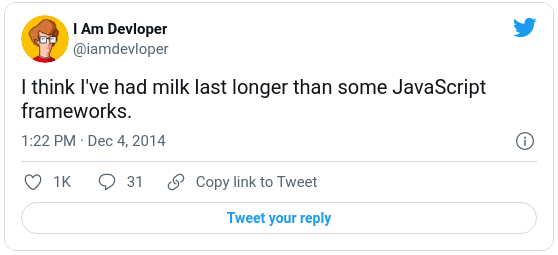
\includegraphics{gfx/js-milk}
    \caption{
        Die Welt der JavaScript Frameworks ändert sich ständig.\cite{twitter-js-state}
        %\footnote{https://twitter.com/iamdevloper/status/540481335362875392}
    }
    \label{fig:frontend-stack}
\end{figure}

Die Debatte, welches Framework denn nun am besten ist, wollen wir in dieser Arbeit nicht behandeln.
Für die Entscheidung welches Frontend Framwork verwendet werden soll, wurde vor allem 'The State of JS'\footnote{https://2020.stateofjs.com/en-US/}
verwendet. The State of JS wertet jedes Jahr verschiedene JavaScript Technologien und Frontend Frameworks
anhand von Entwicklerumfragen aus.\cite{state-of-js-2020-fwk}




